\documentclass[tikz]{standalone}

\usepackage{tikz}
\usepackage{xcolor}
\usepackage{pgfplots}
\usepackage{siunitx}
\usepackage{fontspec}

\pgfplotsset{compat=1.18}

\usetikzlibrary{shapes,arrows,positioning,backgrounds,calc,intersections,calc,svg.path,fit,plotmarks}

\definecolor{ugent-re}{RGB}{220, 78, 40}        % vermilion			/ vermiljoen
\definecolor{ugent-we}{RGB}{45, 140, 168}       % no match
\definecolor{ugent-we-dark}{RGB}{31, 98, 118}       % no match
\definecolor{ugent-ge}{RGB}{232, 94, 113}       % rose				/ bleekrood
\definecolor{ugent-ea}{RGB}{111, 113, 185}      % distant blue		/ verblauw
\definecolor{ugent-pp}{RGB}{251, 126, 58}       % deep orange		/ dieporanje
\definecolor{ugent-ps}{RGB}{113, 168, 96}       % yellow green		/ geelgroen

\begin{document}
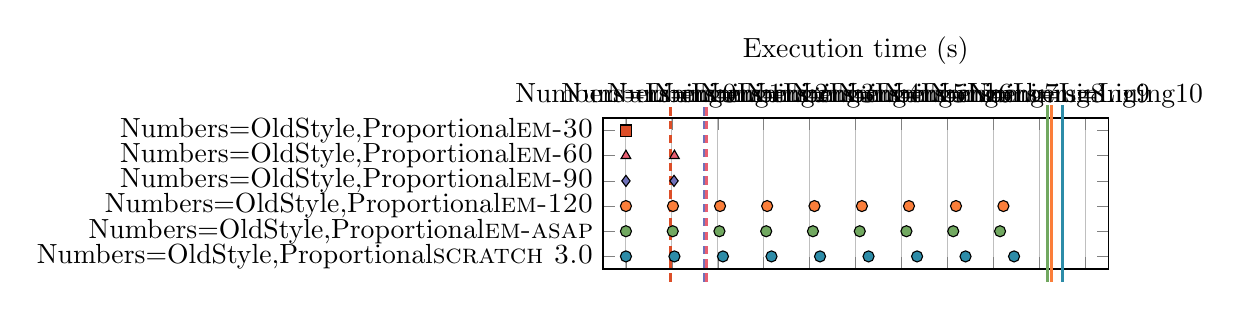
\begin{tikzpicture}
    \pgfplotsset{
        scratch/.style={fill=ugent-we},
        em-30/.style={fill=ugent-re},
        em-60/.style={fill=ugent-ge},
        em-90/.style={fill=ugent-ea},
        em-120/.style={fill=ugent-pp},
        em-asap/.style={fill=ugent-ps},
    }
    \begin{axis}[
        height=3.5cm,
        width=8cm,
        symbolic y coords={min,scratch 3.0,em-asap,em-120,em-90,em-60,em-30,max},
        xtick distance=1000,
        ytick distance=1,
        xmajorgrids,
        xmax=10500,
        xmin=-500,
%        mark size=1pt,
        scaled x ticks=false,
        clip=false,
        xticklabel pos=top,
        xlabel near ticks,
%        extra x ticks={0},
        xlabel={Execution time (s)},
%        ytick pos=bottom,
%        xtick style={draw=none},
%        axis line style={draw=none},
        yticklabel={\addfontfeature{Numbers={OldStyle,Proportional}}\textsc{\tick}},
        xticklabel={\addfontfeature{Numbers={Lining}}\num[round-mode=places,round-precision=0,fixed-exponent=3,exponent-mode=fixed,drop-exponent=true]{\tick}},
%        xticklabel={\addfontfeature{Numbers={OldStyle,Proportional}}\textsc{\tick}}
    ]
        % em-120
        \addplot[em-120,only marks] coordinates {
            (0.0,em-120)
            (1023.7000000476837,em-120)
            (2047.6000000238419,em-120)
            (3073.300000011921,em-120)
            (4103.300000011921,em-120)
            (5135.800000011921,em-120)
            (6159.900000035763,em-120)
            (7183.900000035763,em-120)
            (8215.800000011921,em-120)
        };
        \draw[color=ugent-pp,line width=1pt] (axis cs:9256,min) -- (axis cs:9256,max);
        \addplot[em-30,only marks,mark=square*] coordinates {
            (0.0,em-30)
        };
        \draw[densely dashed,color=ugent-re,line width=1pt] (axis cs:976,min) -- (axis cs:976,max);
        \addplot[em-60,only marks,mark=triangle*] coordinates {
            (0.0,em-60)
            (1055.4000000357628,em-60)
        };
        \draw[densely dashed,color=ugent-ge,line width=1pt] (axis cs:1754,min) -- (axis cs:1754,max);
        \addplot[em-90,only marks,mark=diamond*] coordinates {
            (0.0,em-90)
            (1046.699999988079,em-90)
        };
        \draw[densely dashed,color=ugent-ea,line width=1pt] (axis cs:1701,min) -- (axis cs:1701,max);
        \addplot[scratch,only marks] coordinates {
            (0.0,scratch 3.0)
            (1055.2999999523163,scratch 3.0)
            (2111.5,scratch 3.0)
            (3167.899999976158,scratch 3.0)
            (4224.299999952316,scratch 3.0)
            (5280.399999976158,scratch 3.0)
            (6337.099999964237,scratch 3.0)
            (7391.299999952316,scratch 3.0)
            (8447.5,scratch 3.0)
        };
        \draw[color=ugent-we,line width=1pt] (axis cs:9510,min) -- (axis cs:9510,max);
        \addplot[em-asap,only marks] coordinates {
            (0.0,em-asap)
            (1018.3000000119209,em-asap)
            (2034.699999988079,em-asap)
            (3052.899999976158,em-asap)
            (4070.0,em-asap)
            (5089.199999988079,em-asap)
            (6104.800000011921,em-asap)
            (7123.800000011921,em-asap)
            (8142.899999976158,em-asap)
        };
    \draw[color=ugent-ps,line width=1pt] (axis cs:9176,min) -- (axis cs:9176,max);
    \end{axis}
\end{tikzpicture}
\end{document}
